\section{Introduction}
\label{sec:introduction}

UV atlases for procedural, generated, and noisy assets are usually judged by geometry-facing proxies: chart count, seam length, packing utilization, and area or angle distortion. Production PBR workflows fail through a different interface. A mesh can have an atlas that looks plausible under these proxies, yet still bake roughness, normals, metallic response, and albedo into texture maps that relight poorly. The visible failure is not a single bad UV triangle; it is a held-out rendering residual that concentrates around charts, mips, and cross-channel seams. Our evaluation covers controlled spot, bunny, Objaverse, and procedural noisy transfer cases, plus five real init shapes from two independent SDS pipelines (Fantasia3D \cite{chen2023fantasia3d}, threestudio \cite{guo2023threestudio}); a larger sweep across Trellis-3D \cite{xiang2024_trellis_structured_3d_latents}, GET3D \cite{gao2022_get3d_generative_model}, and DreamFusion-style outputs \cite{poole2023_dreamfusion_text_to_3d} is left to future work.

This mismatch matters because recent UV methods for generated and noisy meshes are increasingly capable at producing compact, part-aware, or learned parameterizations. PartUV reduces chart fragmentation with part-aligned charts \cite{wang2025_partuv_part_based_uv}; FlexPara learns flexible neural surface parameterizations \cite{zhao2025_flexpara_flexible_neural_surface}; and OT-UVGS frames UV assignment for Gaussian splatting as a capacity-allocation problem \cite{kim2026_ot_uvgs_revisiting_uv}. These directions improve or reframe the geometry of the parameterization. They do not directly answer a deployment question faced by asset pipelines: after a fixed single UV set has been produced, should the atlas be locally changed because the baked PBR appearance fails under held-out relighting, or should it be left untouched?

The fixed-atlas condition is practical rather than artificial. In a production asset pipeline, the upstream atlas is often already tied to semantic chart structure, authoring history, part editing, accessory swaps, or animation rigging. A part-aware atlas from PartUV can preserve meaningful chart alignment even when a global xatlas re-chart reports higher relit PSNR on our controlled assets. Switching to xatlas in that situation may discard the part-level structure the pipeline intended to keep. Our goal is therefore to repair an upstream atlas without replacing it, preserving its semantic chart organization whenever the residual evidence justifies a local edit.

We study this question through a deliberately narrow method: a differentiable PBR baking-error atlas. Given a mesh, an initial atlas from a production or learned UV system, and a fixed texture budget, we bake PBR channels, render held-out views and lights, and attribute the residual back to faces, charts, seams, and mip boundaries. The method then proposes local chart repairs and texel reallocations only for residual-heavy regions. A C5 deployment gate evaluates the candidate under matched settings and deploys it only when the relit error and seam evidence improve. If the evidence is insufficient, the final output is the baseline atlas.

\begin{figure*}[t]
  \centering
  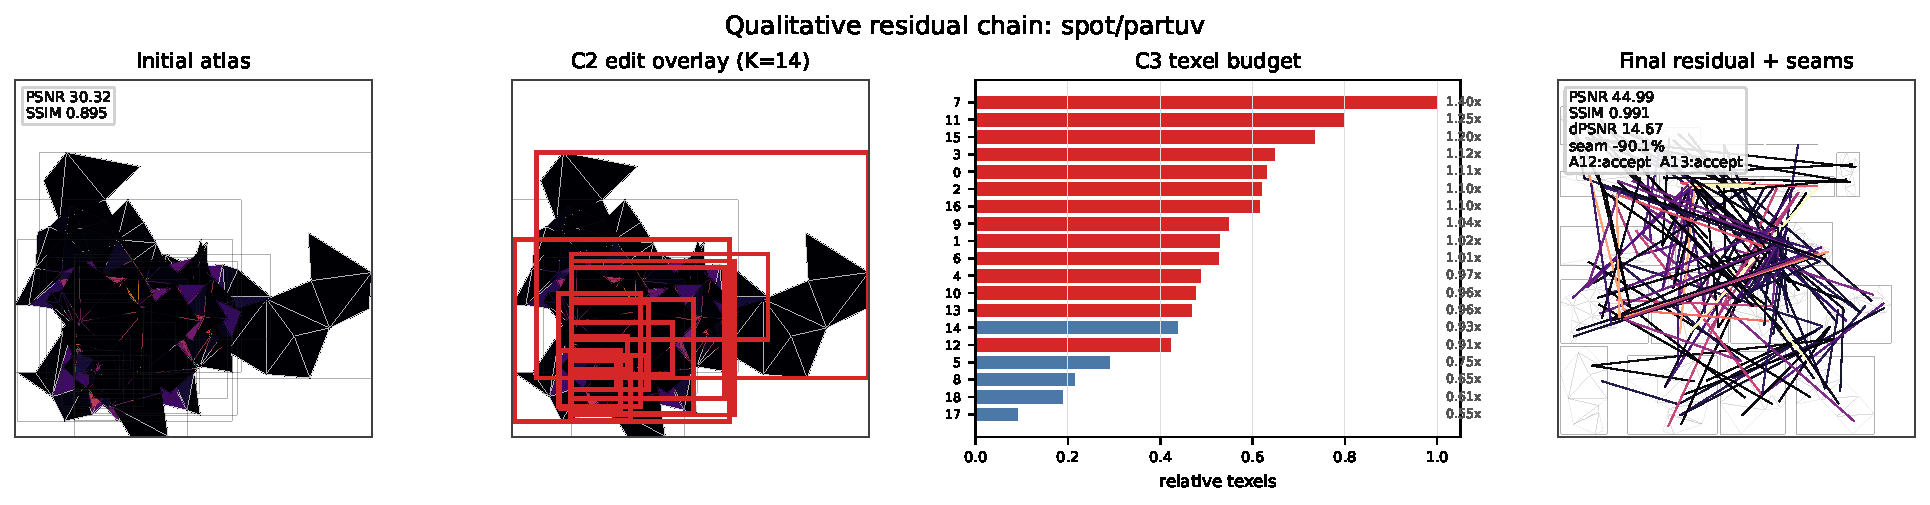
\includegraphics[width=0.92\linewidth]{figures/qualitative_residual_chain/spot_partuv_residual_chain.pdf}
  \caption{PBR baking residual exposes a failure mode of a part-aware atlas. Starting from a PartUV atlas for spot, the differentiable baker localizes held-out relighting residuals, the repair loop edits only selected charts, texel allocation shifts the fixed budget toward residual-heavy regions, and C5 accepts the candidate only when the deployment metrics improve. In this case, relit \PSNR{} improves from 30.32 dB to 44.99 dB; cases without sufficient residual evidence are rolled back.}
  \label{fig:spot_chain}
\end{figure*}

\Cref{fig:spot_chain} shows the intended use case. The initial PartUV atlas for spot has few, semantically coherent charts, but its PBR bake leaves residual structure under relighting. Our repair does not replace PartUV with a new global unwrap. It edits the charts selected by the residual atlas, reallocates texels under the same atlas-size budget, and accepts the result only when held-out relighting improves. This is the core story of the paper: the method is not designed to beat xatlas or oracle UVs when those atlases are already adequate; it is designed to detect and repair the cases where UV proxy metrics miss downstream PBR failure.

Our experiments reflect this deployment stance. On 12 main asset/baseline combinations, C5 accepts only two repairs: spot/PartUV improves by +14.67 dB and bunny/PartUV improves by +10.23 dB. The remaining ten combinations roll back to their baseline atlases, so no deployed row is harmed. On eight procedural noisy transfer assets, the method accepts one additional case, warped cylinder, with +10.74 dB. The cumulative headline trigger rate is therefore 3/20, or 15\%. A supplemental procedural sweep on ten meshes (\cref{tab:transfer_extended}) reproduces this selectivity with one new acceptance (proc\_crumpled\_box, +9.65 dB) and re-confirms warped cylinder; we keep the headline 3/20 separate from the supplemental count to avoid double-reporting overlapping rows. This low trigger rate is a feature of the gate, not a hidden failure of the evaluation: when xatlas, Blender Smart UV, matched oracle, or already adequate PartUV atlases leave no residual-backed room for repair, the method should do nothing.

The strongest caveat is equally central. A strict matched-control study shows that the accepted gains survive atlas-size, padding, and chart-count locks, but vanish when distortion tail or texture utilization are fully locked. The method therefore pays a local price in classical UV proxies to buy PBR fidelity. We expose this trade-off rather than treating it as a confound. Distortion and utilization are important engineering metrics, but they are not the same objective as relit PBR appearance.

This paper makes four contributions. We also report an additional cross-channel seam diagnostic transparently despite its limited isolated signal in the present ablation hooks.
\begin{itemize}
  \item We introduce a differentiable PBR baking-error atlas that attributes held-out relighting residuals to faces, charts, seams, and mip leakage under a standard single UV set.
  \item We propose a constrained local chart repair and texel reallocation loop that operates on an existing atlas rather than replacing the upstream UV method.
  \item We define a C5 deployment gate that accepts only residual-backed PBR improvements and rolls back otherwise, preventing accepted degradation in our tested cases.
  \item We provide an honest matched-control analysis showing that the gains are selective and require localized distortion/utilization freedom, not larger texture budgets, more padding, or more charts.
\end{itemize}

The remainder of the paper follows this evidence chain: \cref{sec:related} positions the work relative to UV parameterization, capacity allocation, and relightable appearance models; \cref{sec:method} defines the residual atlas and repair loop; \cref{sec:experiments} reports the main results, ablations, transfer, and robustness; and \cref{sec:confounds} isolates the trade-offs and limitations of the claims.
